\documentclass[11pt]{article}
\usepackage[margin=1in]{geometry}

\usepackage{amsmath,amssymb}
\usepackage{array}
\usepackage{booktabs}
\usepackage{enumitem}
\usepackage{graphicx}
\usepackage{microtype}
\usepackage{multirow}
\usepackage{url}

\setlength{\parindent}{0pt}
\setlength{\parskip}{0.75\baselineskip}

\title{Robust Hand Landmark Correction via MuJoCo-Constrained Temporal Optimization}
\author{Jiating Li}
\date{\today}

\begin{document}
\maketitle

\begin{abstract}
MediaPipe hand landmarks are convenient to use, but in practice they can become unstable under self-occlusion, oblique viewpoints, and rapid finger motion. We study whether these noisy observations can be improved before downstream gesture recognition by refining them in the actuator space of an articulated ORCA hand model. The proposed method combines a rule-based actuator initialization with MuJoCo-constrained optimization, robust landmark fitting, palm-normal alignment, prior regularization, and first- and second-order temporal consistency terms. Unlike ordinary coordinate-space smoothing, the refinement is carried out in a structured actuator space and checked through MuJoCo forward kinematics. On the current six-class Chinese dance gesture subset, the refined actuator representation gives strong few-shot sequence classification results across several lightweight classifiers, reaching 0.9542 accuracy with SVM and 0.9167 with MLP. At the same time, a RandomForest comparison shows that PCA-reduced raw landmarks remain a strong baseline, reaching 0.9458 accuracy. Overall, the results suggest that actuator-space refinement provides a stable and interpretable representation, while low-dimensional compression of raw landmarks can retain complementary discriminative information.
\end{abstract}

\section{Introduction}
MediaPipe provides a practical real-time pipeline for hand landmark detection and lightweight tracking. It is easy to deploy and works well enough for many interactive tasks, which is why it is often used as the front end in gesture-recognition systems. In our own experiments, however, the landmark sequence is not always stable. Under self-occlusion, oblique viewpoints, or fast finger motion, the predicted keypoints can jitter from frame to frame, drift away from the underlying pose, or briefly move into configurations that do not look anatomically reasonable.

This becomes a problem when the landmarks are used directly for dynamic gesture classification. The downstream model does not see the true hand state; it only sees a sequence of estimated coordinates. If those coordinates are noisy, the sequence representation can mix actual gesture information with artifacts from the visual front end.

Many MediaPipe-based pipelines concentrate on what happens after landmark extraction, for example by adding a temporal encoder or a sequence classifier. In this paper we look one step earlier. Our interest is not mainly in designing a new temporal classifier, but in asking whether the landmark sequence itself can be made more reliable before recognition.

More specifically, we ask whether the structural prior of the ORCA hand, together with the MuJoCo forward model, can be used to convert noisy landmark observations into a cleaner latent representation that is more useful for few-shot gesture recognition.

Our focus is therefore fourfold:
\begin{itemize}[leftmargin=*]
    \item whether raw MediaPipe landmarks are sufficiently stable for sequence recognition;
    \item whether the ORCA actuator space provides a better low-dimensional and structured representation;
    \item whether MuJoCo-constrained optimization further mitigates transient landmark drift; and
    \item whether a smoother latent actuator trajectory improves downstream few-shot sequence classification.
\end{itemize}

The paper is therefore organized around causal frame-wise latent-state refinement as the main method, while sequence aggregation and classification are used only for downstream evaluation.

An important part of the paper is to distinguish this approach from simpler alternatives. Since the target problem is temporal instability in estimated landmark sequences, the first question is whether standard landmark-space smoothing would already be enough. We therefore compare against several ordinary filtering baselines. The second question is whether any improvement comes mostly from dimensionality reduction rather than from the ORCA/MuJoCo structure itself. This motivates a separate comparison against PCA-reduced raw landmarks. The experiments are arranged with these two questions in mind.

Accordingly, this paper should be read as a MuJoCo-constrained refinement framework for improving the robustness of MediaPipe landmark sequences, rather than as a new temporal gesture classifier.

The main contributions of this work are as follows:
\begin{itemize}[leftmargin=*]
    \item We introduce a structured landmark-refinement pipeline that maps noisy MediaPipe observations into the actuator space of an articulated ORCA hand model.
    \item We formulate MuJoCo-constrained temporal optimization with robust landmark fitting, prior regularization, and acceleration-aware temporal consistency to obtain a stable latent actuator representation.
    \item We show that the refined latent representation improves downstream few-shot dynamic gesture classification relative to raw landmarks, heuristic actuator-space projection, and PCA-reduced baselines. Within the actuator space, the optimized representation also exhibits reduced temporal variation relative to the heuristic projection baseline.
\end{itemize}

\section{Related Work}
\subsection{Vision-based Hand Keypoint Estimation}
Modern vision-based hand trackers provide convenient 2D/3D keypoints together with lightweight frame-to-frame tracking, but they still struggle in the cases that matter most for articulated hands: self-occlusion, severe perspective change, and fast local motion. In such cases, the predicted landmarks may look acceptable in a single frame while remaining unstable over time. This is especially problematic when the landmarks are used directly for downstream recognition or control.

\subsection{Physical and Kinematic Constraints for Pose Correction}
A common way to improve noisy pose observations is to introduce priors from kinematic structure, embodiment, inverse kinematics, or temporal consistency. Instead of smoothing coordinates directly, these approaches try to regularize the solution in a lower-dimensional configuration space where implausible states are easier to reject. Our method follows this general idea, but does so in the actuator space of an embodied ORCA hand and checks candidate configurations through MuJoCo forward kinematics.

\subsection{Few-shot Gesture Recognition}
Few-shot gesture recognition is particularly sensitive to representation quality, because there is limited data to average out nuisance variation. Many practical landmark-based pipelines treat extracted keypoints as ready-to-use temporal features and concentrate on recurrent or transformer-style sequence models. Our emphasis is different. We are interested in whether a better frame-level representation, obtained before temporal modeling, can already improve downstream recognition in a low-data setting. This is the main reason for using actuator-space features together with lightweight sequence-level classifiers in the present evaluation.

\section{Method}
Let $\mathbf{y}_t \in \mathbb{R}^{21 \times 3}$ denote the MediaPipe hand landmarks at frame $t$, and let the vectorized form also be written as $\mathbf{y}_t \in \mathbb{R}^{63}$. Our goal is to transform these noisy observations into a stable latent actuator trajectory $\mathbf{q}_t^* \in \mathbb{R}^{17}$ that is kinematically plausible under the ORCA hand structure and MuJoCo forward kinematics.

\subsection{Raw Hand Landmark Extraction}
We begin from the normalized $21 \times 3$ landmarks predicted by MediaPipe. These landmarks serve as the raw observation space and directly capture wrist pose, finger articulation, and hand shape. However, because the representation is high-dimensional and unconstrained, it is sensitive to frame-level estimation noise and can fluctuate even when the underlying gesture remains unchanged.

\subsection{Embodiment-aware Actuator-space Projection}
The first structured representation is a rule-based projection from landmarks to the ORCA actuator space:
\[
\tilde{\mathbf{q}}_t = g(\mathbf{y}_t), \qquad \tilde{\mathbf{q}}_t \in \mathbb{R}^{17}.
\]
Here, $g(\cdot)$ is a hand-designed geometric mapping that extracts semantically meaningful quantities such as wrist orientation, finger flexion, finger abduction, thumb opening, and palm normal direction. This representation, referred to as \texttt{corrected}, is not learned and is not obtained by optimization. Instead, it is an embodiment-constrained reparameterization that replaces high-dimensional landmark coordinates with a low-dimensional semantic actuator description.

The advantage of \texttt{corrected} is interpretability and structural compactness, which can already benefit few-shot classification. Its limitation is that it is computed independently for each frame and therefore does not explicitly suppress temporal jitter.

\subsection{MuJoCo-constrained Causal Temporal Refinement}
To obtain a more stable latent state, we optimize actuator variables against the observed landmarks while enforcing kinematic consistency through MuJoCo forward kinematics. In this sense, the refinement is physics-informed: candidate states are regularized by a simulated articulated hand model rather than by coordinate-space smoothing alone. Let $h(\mathbf{q})$ denote the MuJoCo forward model that maps actuator states to landmark positions, and let $\mathcal{Q}$ denote the feasible actuator set.

The optimized action representation solves
\[
\mathbf{q}_t^*
=
\arg\min_{\mathbf{q}_t \in \mathcal{Q}}
\lambda_l \mathcal{L}_{\text{huber}}
+
\lambda_n \mathcal{L}_{\text{normal}}
+
\lambda_p \mathcal{L}_{\text{prior}}
+
\lambda_s \mathcal{L}_{\text{temporal}}
+
\lambda_a \mathcal{L}_{\text{acceleration}}
+
\lambda_d \mathcal{L}_{\text{default}}
+
\lambda_b \mathcal{L}_{\text{boundary}}.
\]
The main fitting and regularization terms are
\[
\mathcal{L}_{\text{huber}}
=
\sum_i \rho_\delta \!\left(\left\| h_i(\mathbf{q}_t) - \mathbf{y}_{t,i} \right\|_2\right),
\qquad
\mathcal{L}_{\text{normal}}
=
\left\| \mathbf{n}_{\text{orca}}(\mathbf{q}_t) - \mathbf{n}_{\text{mp}}(\mathbf{y}_t) \right\|_2^2,
\]
\[
\mathcal{L}_{\text{prior}}
=
\left\| \mathbf{q}_t - \tilde{\mathbf{q}}_t \right\|_2^2,
\qquad
\mathcal{L}_{\text{temporal}}
=
\left\| \mathbf{q}_t - \mathbf{q}_{t-1}^* \right\|_2^2.
\]
The Huber penalty for a residual $r$ is
\[
\rho_{\delta}(r)
=
\begin{cases}
\frac{1}{2} r^2, & |r| \le \delta, \\
\delta \left(|r| - \frac{1}{2}\delta\right), & |r| > \delta,
\end{cases}
\]
which behaves like an $L_2$ loss for small residuals and like an $L_1$-style penalty for large residuals. This reduces the influence of transient MediaPipe failures. We also add an acceleration regularizer,
\[
\mathcal{L}_{\text{acceleration}}
=
\left\| \mathbf{q}_t - 2\mathbf{q}_{t-1}^* + \mathbf{q}_{t-2}^* \right\|_2^2,
\]
which penalizes abrupt second-order changes in the actuator trajectory. The resulting representation is best interpreted as a robust temporally regularized latent-state estimator rather than a simple smoother.

For visualization and geometric evaluation, we further reconstruct a landmark representation by projecting the optimized actuator state back through MuJoCo:
\[
\mathbf{y}_t^* = h(\mathbf{q}_t^*).
\]
We refer to this reconstructed landmark sequence as \texttt{optimized\_full}. Although it is useful for assessing geometric consistency, it is not necessarily the best representation for classification because it returns to a higher-dimensional coordinate space.

\subsection{Sequence-level Statistical Aggregation for Downstream Evaluation}
The main method operates at the frame level. For downstream few-shot classification, we aggregate frame-wise features across a sequence using summary statistics such as mean, standard deviation, maximum, and temporal difference descriptors. If a frame-level feature is $\mathbf{x}_t \in \mathbb{R}^{d}$, then for a sequence of length $T$ we compute
\[
\boldsymbol{\mu} = \frac{1}{T}\sum_{t=1}^{T}\mathbf{x}_t,\qquad
\boldsymbol{\sigma} = \mathrm{std}(\mathbf{x}_1,\dots,\mathbf{x}_T),
\]
\[
\mathbf{m} = \max_{t=1,\dots,T}\mathbf{x}_t,\qquad
\boldsymbol{\Delta} = \mathbf{x}_T - \mathbf{x}_1,
\]
and concatenate them into
\[
\mathbf{z}^{(s)} = [\boldsymbol{\mu}, \boldsymbol{\sigma}, \mathbf{m}, \boldsymbol{\Delta}] \in \mathbb{R}^{4d}.
\]
This aggregation is an evaluation protocol rather than the correction method itself. Its purpose is to compare whether cleaner frame-level representations lead to better sequence-level classification under limited supervision.

We intentionally adopt this lightweight statistical sequence encoding for two reasons. First, it keeps the downstream model simple enough that any gain can be attributed mainly to representation quality rather than to a high-capacity temporal classifier. Second, in the current few-shot setting, a compact fixed-length descriptor provides a reasonable bias--variance tradeoff and avoids over-interpreting short and noisy training sequences. Stronger temporal baselines such as GRU and LSTM remain important future comparisons, but they are not necessary for establishing the main point of this paper, namely frame-level landmark refinement in a structured actuator space.

\begin{table}[t]
\centering
\caption{Summary of the representations used in this study.}
\footnotesize
\renewcommand{\arraystretch}{1.15}
\begin{tabular}{@{}>{\raggedright\arraybackslash}p{0.20\linewidth} >{\raggedright\arraybackslash}p{0.06\linewidth} >{\raggedright\arraybackslash}p{0.15\linewidth} >{\raggedright\arraybackslash}p{0.10\linewidth} >{\raggedright\arraybackslash}p{0.10\linewidth} >{\raggedright\arraybackslash}p{0.22\linewidth}@{}}
\toprule
Representation & Dim. & Source & Optimized & Temporal & Main role \\
\midrule
\texttt{corrected} & 17 & geometric mapping & no & no & structured low-dimensional feature \\
\texttt{optimized\_action} & 17 & robust MuJoCo optimization & yes & strong & stable and discriminative latent state \\
\texttt{optimized\_full} & 63 & forward reconstruction & indirect & inherited & structure-consistent landmark reconstruction \\
\bottomrule
\end{tabular}
\end{table}

\section{Experiments and Results}
\subsection{Dataset and Gesture Classes}
We evaluate the method on the current sequence dataset \texttt{gesture\_sequence\_dataset\_optimized\_v2.csv} and focus the main experimental analysis on a six-class Chinese dance subset filtered from the full collection. The six gesture classes are \texttt{orchid\_palm}, \texttt{orchid\_finger}, \texttt{flower\_pinch}, \texttt{prayer\_beads}, \texttt{three\_finger\_bent}, and \texttt{deer\_horn}. This subset is used as the primary task because it reflects the intended fine-grained application domain of the work. We retain the broader mixed-gesture results only as supplemental evidence that the representation generalizes beyond the targeted dance gesture set.

The downstream evaluation follows a few-shot setting with three training sequences per class, and each experiment is repeated 20 times with different train/test splits. Because the current dataset is still moderately imbalanced across classes, we report multiple metrics beyond accuracy, including macro-F1 and Cohen's kappa.

\subsection{Frame-level Stability Evaluation}
Frame-level evaluation focuses on jitter, drift, and transient outliers. Beyond comparing raw landmarks, heuristic actuator projections, and optimized actuator states, we additionally include conventional temporal smoothing baselines, including moving average, Savitzky--Golay, One-Euro, and Kalman filtering. The purpose of these baselines is to test whether the observed benefits could be explained by coordinate-space denoising alone. Because these baselines operate directly in landmark space, they are compared primarily against raw landmarks and the reconstructed landmark output of the proposed method.

We evaluate temporal smoothness separately in actuator space and landmark space. This distinction is important because the latent actuator trajectory and the reconstructed landmark trajectory live in different spaces, with different dimensionalities and scales. Within each space, lower velocity- and acceleration-based statistics indicate smoother temporal behavior.

\begin{table}[t]
\centering
\caption{Actuator-space temporal stability on the current dataset. Lower is better.}
\label{tab:jitter_actuator}
\small
\begin{tabular}{@{}lcccc@{}}
\toprule
Representation & Velocity Mean & Velocity RMS & Acceleration Mean & Acceleration RMS \\
\midrule
Corrected & 0.6215 & 0.8251 & 0.9509 & 1.2118 \\
Optimized Action & \textbf{0.3343} & \textbf{0.4190} & \textbf{0.3580} & \textbf{0.4517} \\
\bottomrule
\end{tabular}
\end{table}

\begin{table}[t]
\centering
\caption{Landmark-space temporal stability on the current dataset. Lower is better.}
\label{tab:jitter_landmark}
\small
\begin{tabular}{@{}lcccc@{}}
\toprule
Representation & Velocity Mean & Velocity RMS & Acceleration Mean & Acceleration RMS \\
\midrule
Raw & \textbf{0.4439} & \textbf{0.5566} & 0.5952 & \textbf{0.7256} \\
Optimized Full & 0.4517 & 0.7190 & \textbf{0.5194} & 0.8169 \\
\bottomrule
\end{tabular}
\end{table}

Within actuator space, \texttt{optimized\_action} has lower velocity and acceleration than the heuristic \texttt{corrected} representation, which suggests that robust fitting and acceleration regularization reduce short-lived drift in the latent trajectory. Within landmark space, \texttt{optimized\_full} can be compared against raw MediaPipe landmarks, but these values should not be compared directly with actuator-space statistics. Taken together, these results support using the refined latent actuator trajectory as the main representation for downstream recognition.

\begin{figure}[t]
\centering
\begin{minipage}[t]{0.48\linewidth}
\centering
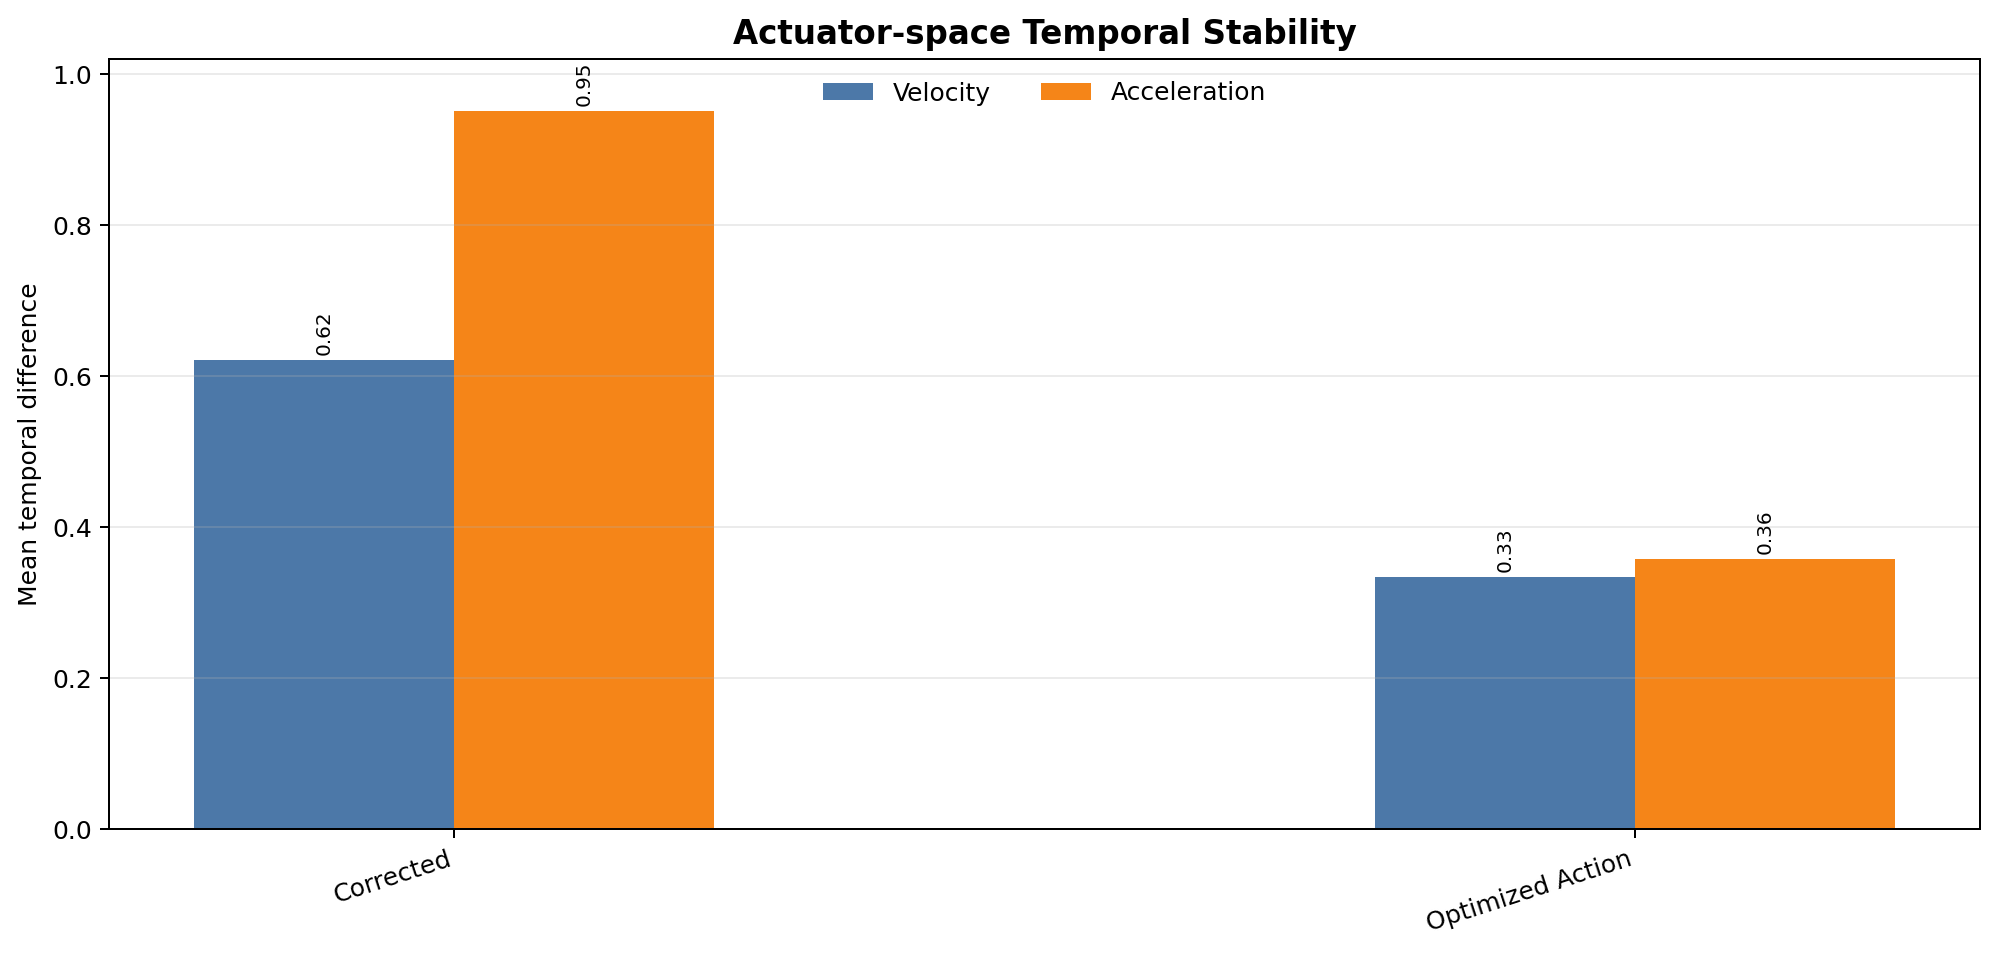
\includegraphics[width=\linewidth]{figures/paper_rewrite_main/jitter_actuator_space.png}
\end{minipage}
\hfill
\begin{minipage}[t]{0.48\linewidth}
\centering
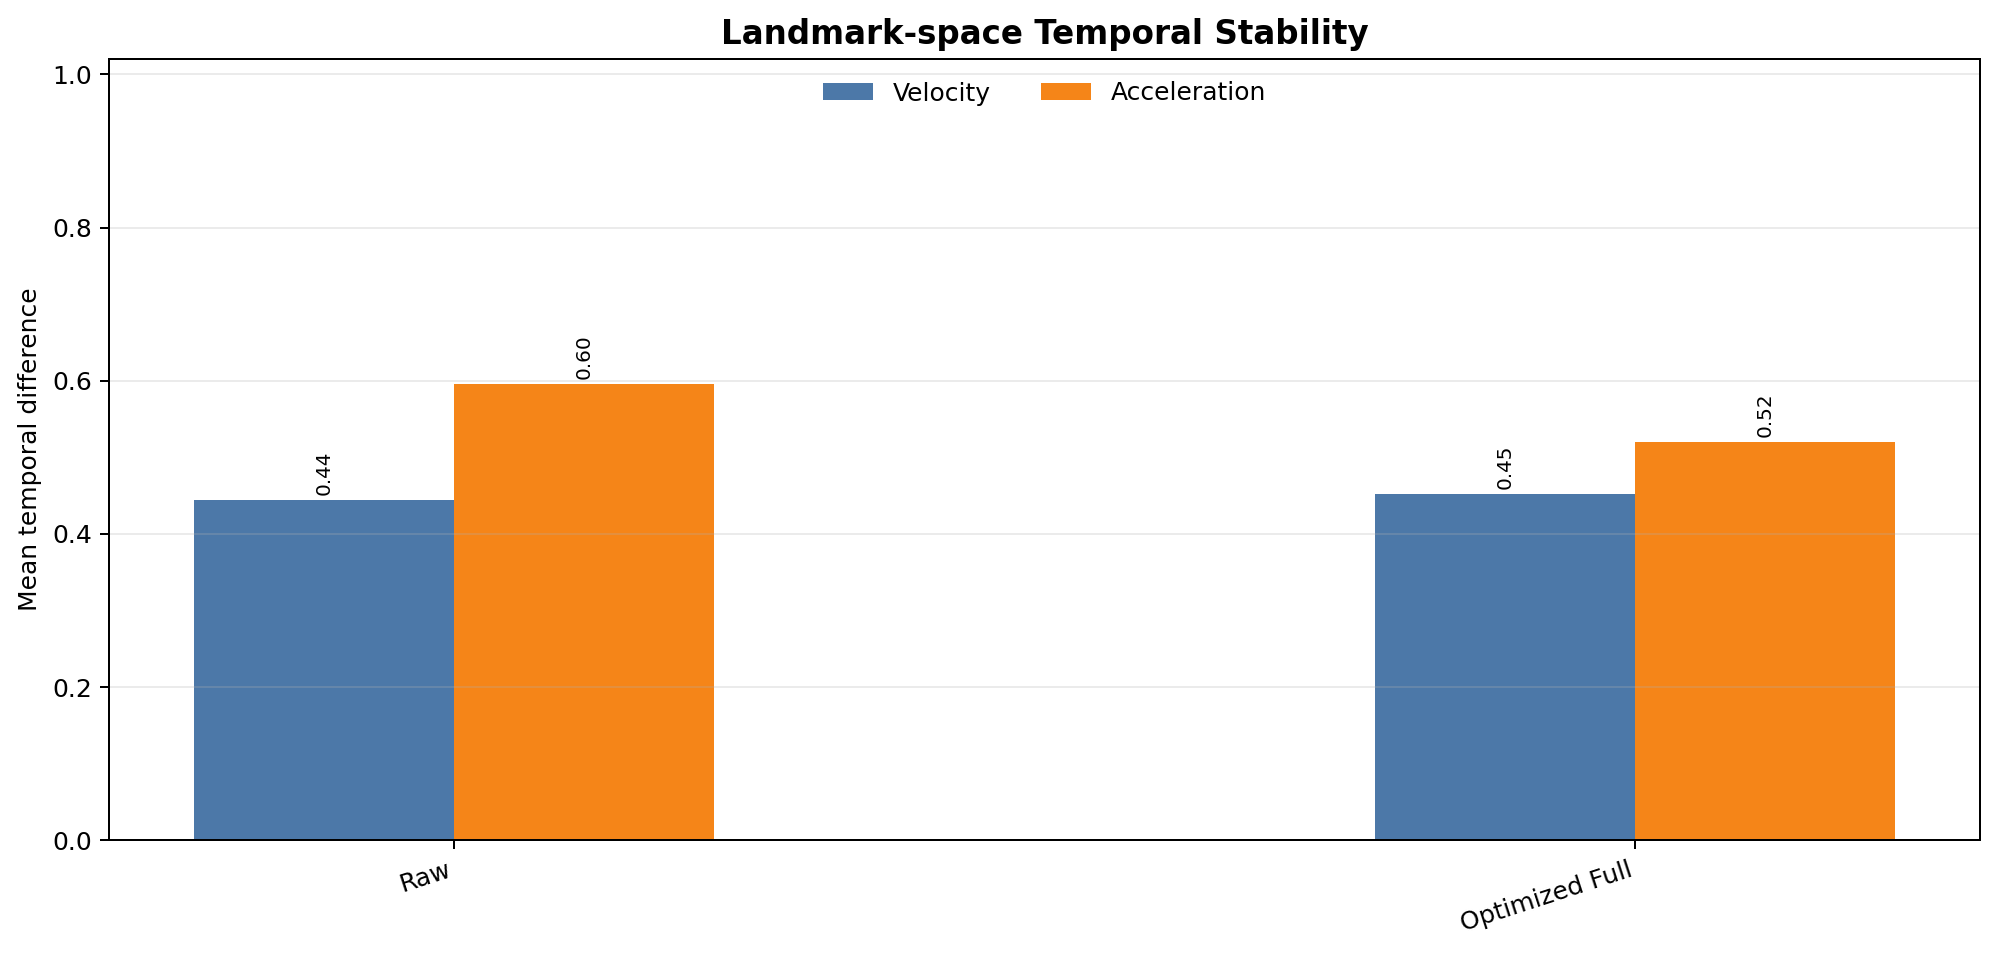
\includegraphics[width=\linewidth]{figures/paper_rewrite_main/jitter_landmark_space.png}
\end{minipage}
\caption{Temporal stability summaries in actuator space and landmark space. The optimized actuator trajectory substantially reduces actuator-space velocity and acceleration relative to the heuristic corrected representation, while landmark-space reconstruction should be interpreted separately because it lives in a different coordinate space.}
\label{fig:jitter_summary}
\end{figure}

\subsection{Sequence-level Few-shot Classification}
To measure downstream utility, we aggregate frame-level features into sequence descriptors and train few-shot classifiers on top of each representation. The main question here is whether a more stable actuator trajectory is also a more discriminative representation under limited training data. The comparisons are organized in two stages. First, we compare against landmark-space smoothing baselines to test whether ordinary temporal filtering is already sufficient. Second, we compare against PCA-reduced baselines to test whether the benefit of actuator-space features can be explained by generic dimensionality reduction.

We next evaluate whether the cleaner frame-level representations lead to better sequence-level few-shot recognition. Table~\ref{tab:main_classifiers} reports the current results across three currently reported lightweight classifiers.

\begin{table}[t]
\centering
\caption{Few-shot sequence classification results on the six-class Chinese dance subset (mean over 20 repeats).}
\label{tab:main_classifiers}
\footnotesize
\begin{tabular}{@{}llccc@{}}
\toprule
Classifier & Representation & Accuracy & Macro-F1 & Kappa \\
\midrule
\multirow{4}{*}{SVM}
& Raw & 0.8250 & 0.7985 & 0.7841 \\
& Corrected & 0.9458 & 0.9262 & 0.9330 \\
& Optimized Action & \textbf{0.9542} & \textbf{0.9378} & \textbf{0.9429} \\
& Optimized Full & 0.7958 & 0.7334 & 0.7468 \\
\midrule
\multirow{4}{*}{RandomForest}
& Raw & 0.8708 & 0.8588 & 0.8413 \\
& Corrected & 0.9083 & 0.8850 & 0.8874 \\
& Optimized Action & 0.9292 & 0.9168 & 0.9130 \\
& Optimized Full & 0.8750 & 0.8676 & 0.8457 \\
\midrule
\multirow{4}{*}{MLP}
& Raw & 0.8208 & 0.7923 & 0.7820 \\
& Corrected & 0.8958 & 0.8781 & 0.8720 \\
& Optimized Action & 0.9167 & 0.9062 & 0.8977 \\
& Optimized Full & 0.7708 & 0.7141 & 0.7162 \\
\bottomrule
\end{tabular}
\end{table}

Across classifiers, \texttt{optimized\_action} is consistently among the strongest representations and is the best structured representation in all three currently reported classifier comparisons. In particular, SVM with \texttt{optimized\_action} reaches 0.9542 accuracy, 0.9378 macro-F1, and 0.9429 Cohen's kappa on the six-class subset. This suggests that the refined actuator representation is not only smoother in latent space, but also more useful for fine-grained gesture recognition.

\begin{figure}[t]
\centering
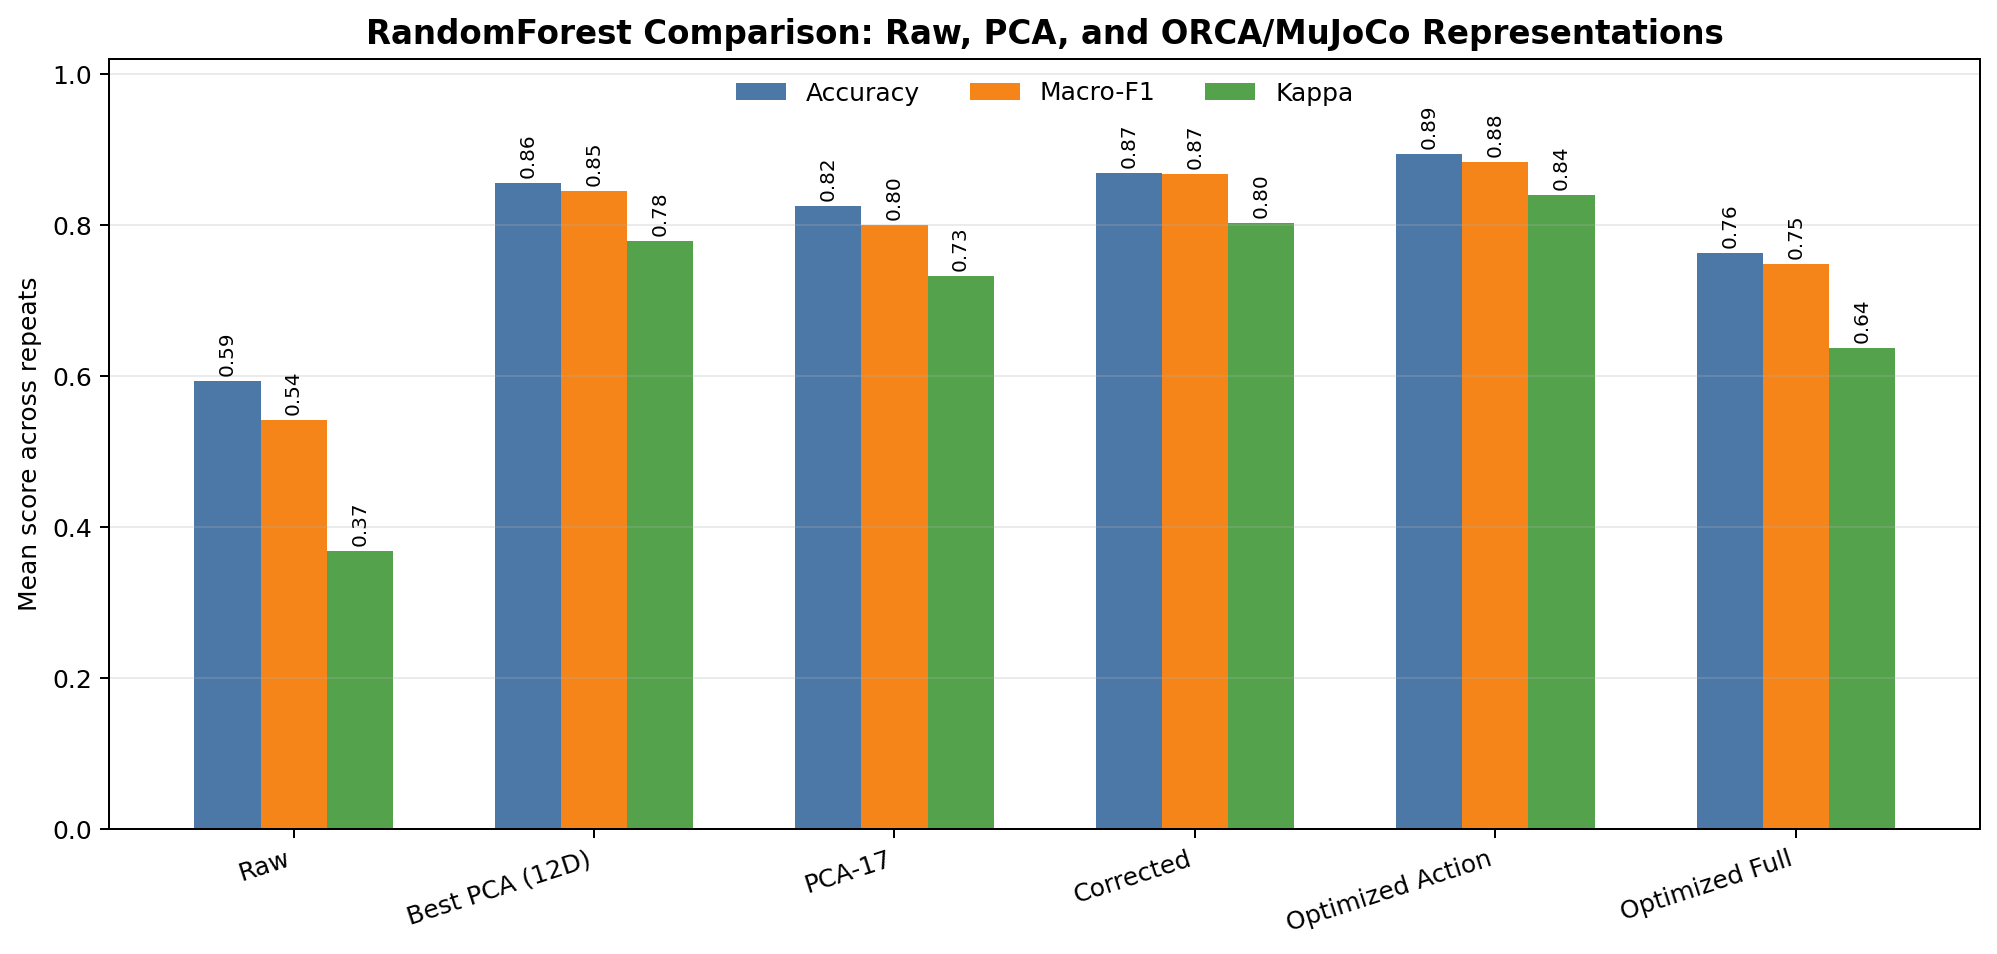
\includegraphics[width=0.86\linewidth]{figures/paper_rewrite_main/representation_comparison.png}
\caption{Six-class representation comparison across raw landmarks, heuristic actuator projection, MuJoCo-refined actuator features, reconstructed landmarks, and PCA-reduced raw landmarks. The refined actuator representation is consistently among the strongest representations, while the PCA baseline remains highly competitive in the current task.}
\label{fig:representation_comparison}
\end{figure}

\subsection{Classifier Comparison}
The classifier comparison suggests two fairly clear observations. First, representation choice matters more than classifier choice when comparing raw landmarks against corrected or optimized representations: all three currently reported classifiers improve once the features become more structured. Second, the refined actuator representation is useful across different lightweight learners rather than being tied to one particular model. In the current six-class setting, SVM gives the strongest overall result for \texttt{optimized\_action}, while RandomForest and MLP show the same overall ranking trend.

\subsection{Ablation-oriented PCA Baseline Analysis}
Because the optimized action space is 17-dimensional, one natural question is whether its advantage comes merely from dimensionality reduction. To test this, we compare against PCA-reduced raw landmarks in two complementary ways: PCA-17 as a dimension-matched baseline, and the best validated PCA baseline selected through a PCA sweep. On the current six-class subset, the strongest PCA comparison is \texttt{raw\_pca17} under RandomForest, which reaches 0.9458 accuracy, 0.9528 macro-F1, and 0.9336 kappa. This result is important because it shows that generic low-dimensional compression remains a very strong baseline for fine-grained hand gesture recognition.

\begin{table}[t]
\centering
\caption{Focused comparison between raw landmarks, PCA baselines, and structured ORCA/MuJoCo representations on the six-class subset.}
\label{tab:rf_pca}
\small
\begin{tabular}{@{}lcccc@{}}
\toprule
Classifier & Representation & Accuracy & Macro-F1 & Kappa \\
\midrule
RandomForest & Raw & 0.8708 & 0.8588 & 0.8413 \\
RandomForest & Best PCA baseline (\texttt{raw\_pca17}) & \textbf{0.9458} & \textbf{0.9528} & \textbf{0.9336} \\
RandomForest & Corrected & 0.9083 & 0.8850 & 0.8874 \\
RandomForest & Optimized Action & 0.9292 & 0.9168 & 0.9130 \\
SVM & Best structured baseline (\texttt{optimized\_action}) & \textbf{0.9542} & \textbf{0.9378} & \textbf{0.9429} \\
\bottomrule
\end{tabular}
\end{table}

This comparison leads to a more balanced conclusion than the earlier three-class results. On the one hand, the PCA baseline confirms that low-dimensional compression alone can already work very well, especially for fine-grained Chinese dance gestures. On the other hand, \texttt{optimized\_action} remains the strongest structured representation and achieves the best overall SVM result. The picture is therefore not simply ``PCA versus not PCA.'' A more accurate reading is that structured actuator-space refinement and low-dimensional geometric compression preserve different useful cues, and their relative strength depends on the downstream classifier.

\begin{figure}[t]
\centering
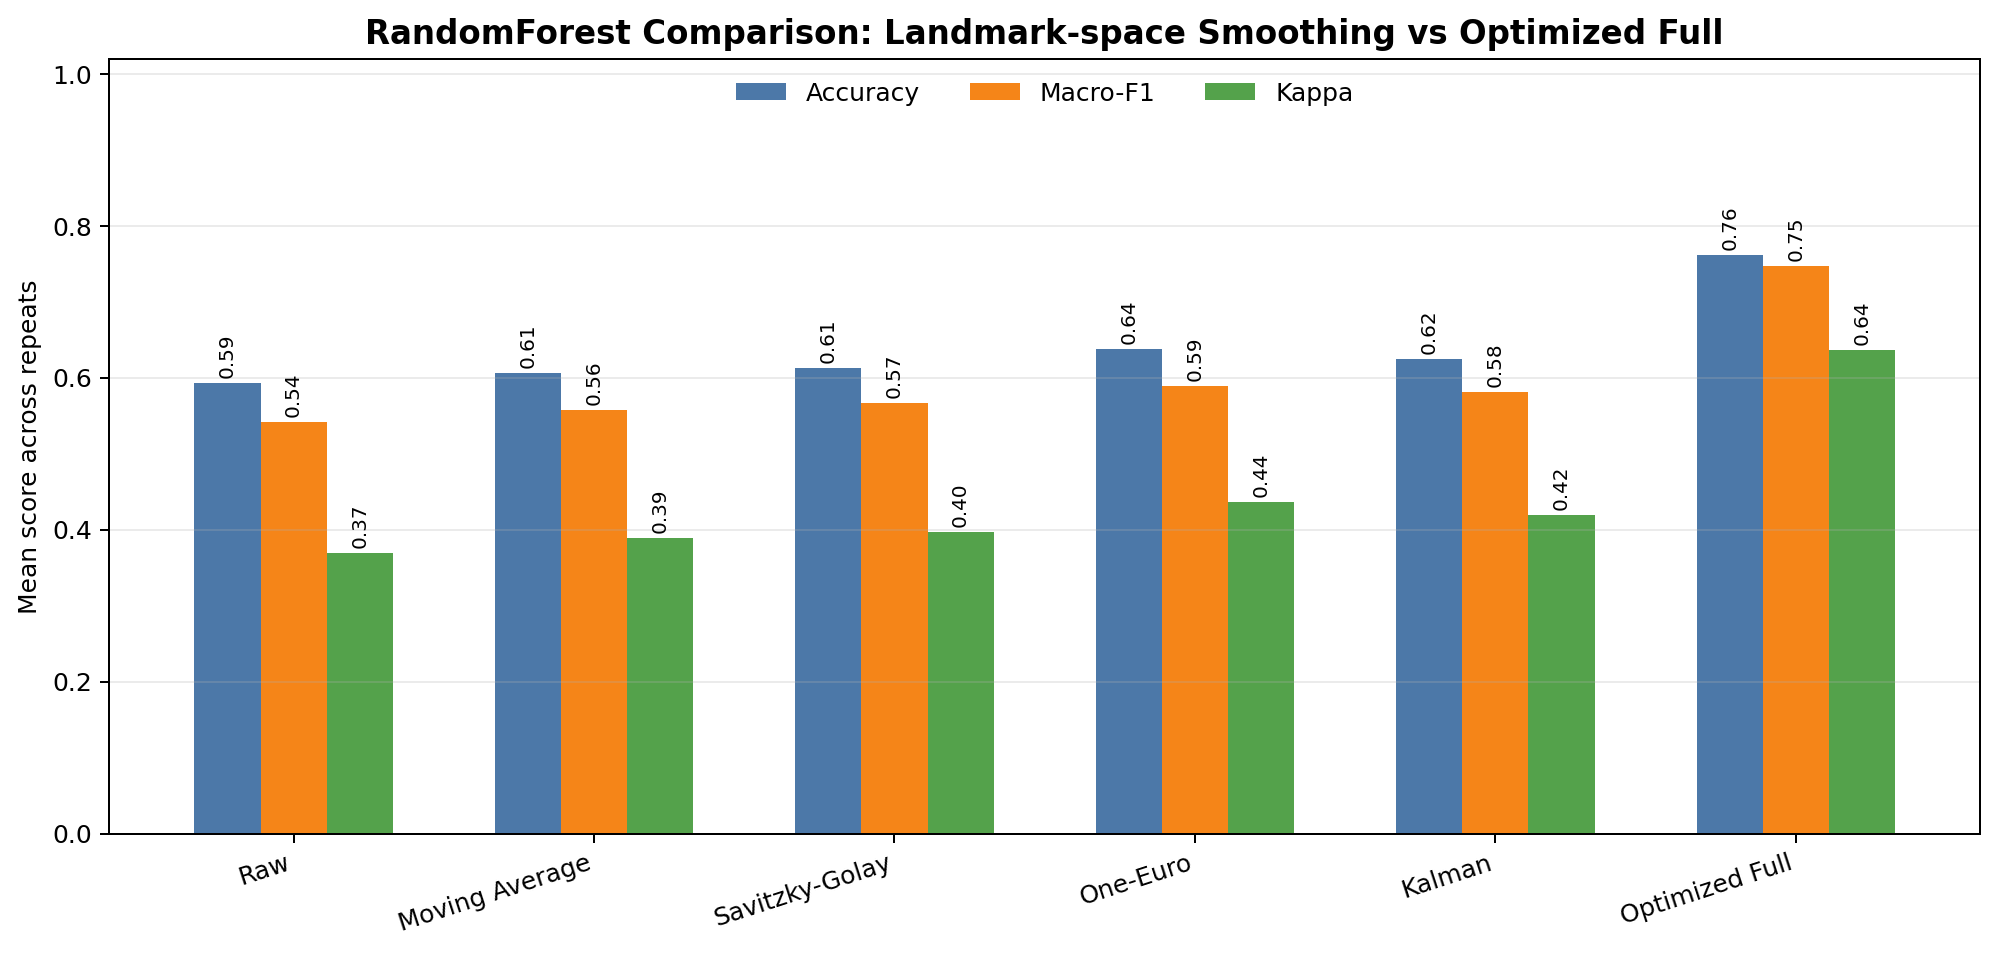
\includegraphics[width=0.86\linewidth]{figures/paper_rewrite_main/smoothing_comparison.png}
\caption{Comparison against conventional smoothing baselines. Ordinary coordinate-space filtering provides only limited improvement over raw landmarks, whereas structured ORCA/MuJoCo-based refinement remains substantially stronger.}
\label{fig:smoothing_comparison}
\end{figure}

\section{Discussion}
\subsection{Why Frame Correction Improves Sequence Classification}
Sequence classifiers depend on stable frame-level evidence. When raw landmarks fluctuate because of viewpoint changes or self-occlusion, the resulting sequence descriptors mix gesture information with estimation noise. By correcting landmarks in actuator space, the proposed method reduces some of this nuisance variation before sequence aggregation.

The smoothing baselines help sharpen this interpretation. If the problem were only high-frequency temporal noise, then conventional coordinate-space filtering would be expected to close most of the gap. In our results, however, smoothing provides only limited gains over raw landmarks, while the structured ORCA/MuJoCo-based representations remain much stronger. This suggests that the dominant errors are not only temporal fluctuations, but also structurally inconsistent local observations that are not handled well by independent per-coordinate filtering.

\subsection{Reconstruction versus Discriminative Representation}
A lower reconstruction error does not necessarily imply better classification. The reconstructed landmark space \texttt{optimized\_full} is useful for visualization and kinematic plausibility checks, but the compact actuator representation \texttt{optimized\_action} is more attractive for few-shot classification because it is lower-dimensional, structured, and more closely aligned with articulation semantics.

The PCA comparison provides a second clarification. Even if a compact representation improves classification, that improvement is not automatically evidence for embodiment-aware refinement, because generic dimensionality reduction can also help in low-data settings. For this reason, PCA baselines are necessary to test whether the benefit comes merely from compression.

The updated six-class results also reveal an important trade-off. Under RandomForest, PCA-compressed raw landmarks can outperform the structured actuator representation, suggesting that a geometry-preserving low-dimensional embedding remains highly effective for this fine-grained task. Under SVM and MLP, however, \texttt{optimized\_action} remains best or tied among the strongest representations. This makes the paper stronger rather than weaker: rather than claiming universal dominance, we can argue more carefully that ORCA/MuJoCo-constrained refinement provides a robust, interpretable, and highly competitive structured alternative to generic dimensionality reduction.

\begin{figure}[t]
\centering
\begin{minipage}[t]{0.48\linewidth}
\centering
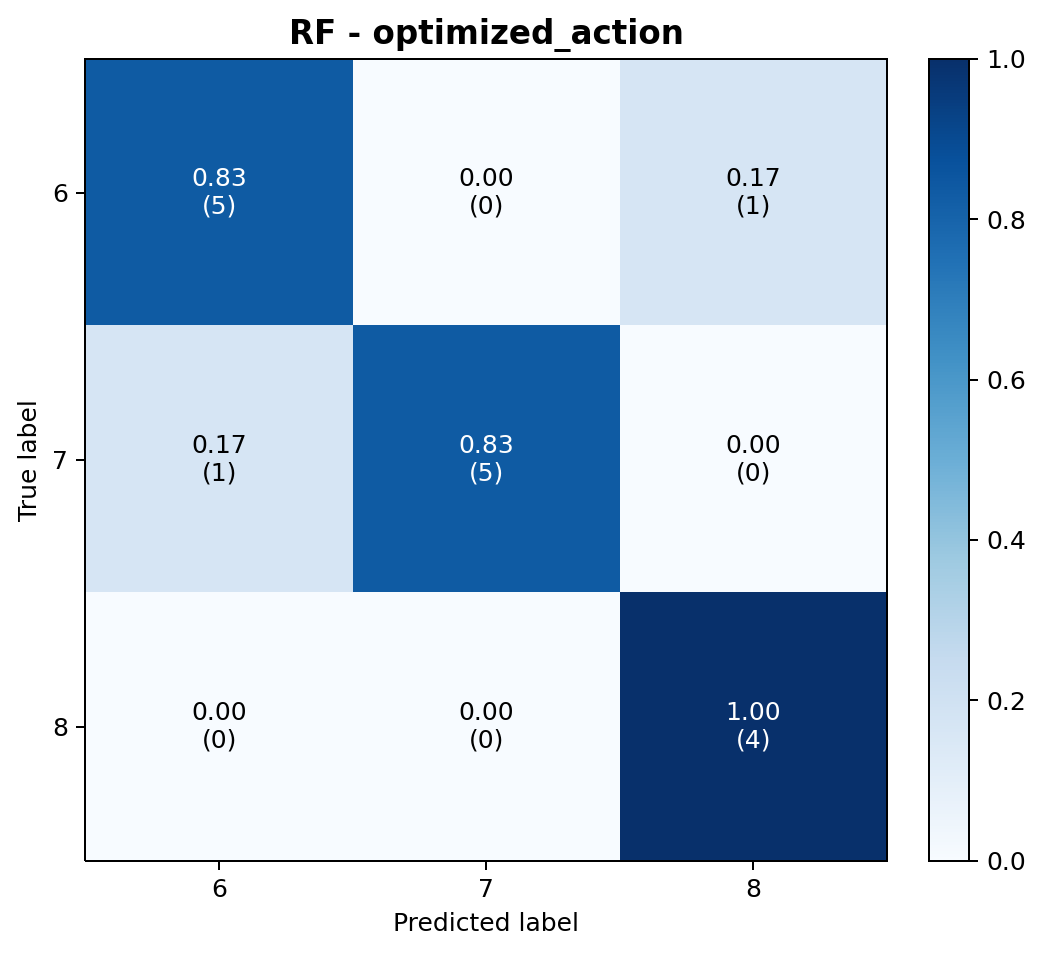
\includegraphics[width=\linewidth]{figures/paper_rewrite_main/best_cm_optimized_action.png}
\end{minipage}
\hfill
\begin{minipage}[t]{0.48\linewidth}
\centering
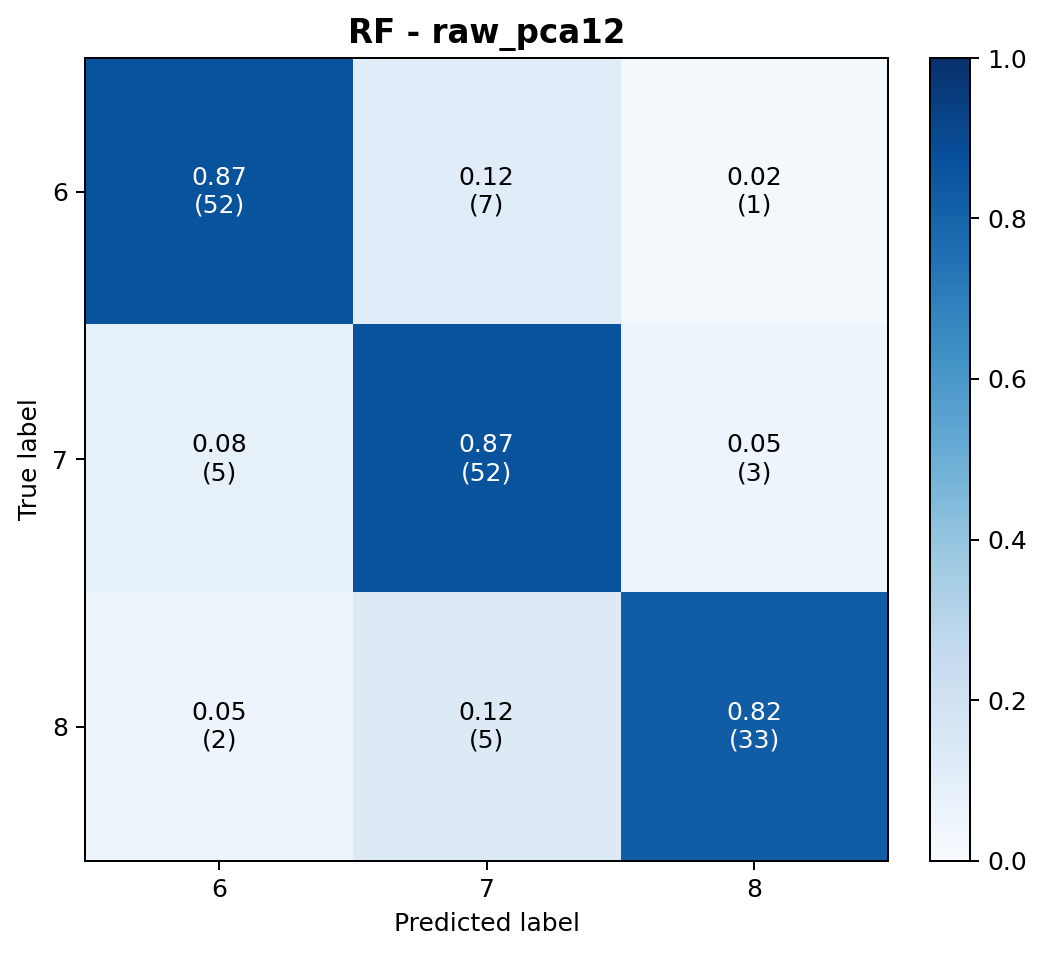
\includegraphics[width=\linewidth]{figures/paper_rewrite_main/best_cm_best_pca.png}
\end{minipage}
\caption{Representative confusion matrices for two strongest configurations in the current study: the optimized actuator representation as the best structured feature set, and the strongest PCA-reduced raw landmark baseline. Together they illustrate that structured actuator refinement and low-dimensional geometric compression provide complementary discrimination patterns.}
\label{fig:best_confusion_matrices}
\end{figure}

\subsection{Limitation of Statistical Aggregation}
Simple statistical aggregation is convenient and easy to interpret, but it discards temporal ordering beyond a few low-order summaries. Stronger sequence models such as recurrent networks or temporal transformers may extract additional discriminative information once a stable frame-level representation is available.

\subsection{Future Work with Stronger Temporal Models}
The current framework isolates the effect of frame-level correction. A natural next step is to combine the refined actuator trajectory with stronger temporal encoders, such as GRU or LSTM baselines, to test whether richer sequence models can further improve recognition accuracy. Another promising direction is cross-session validation with more gesture classes and larger subject diversity.

\section{Conclusion}
We present a MuJoCo-constrained temporal optimization framework for correcting noisy hand landmarks in an ORCA actuator space. The method goes beyond conventional temporal smoothing by incorporating embodiment priors, forward-kinematic consistency, robust fitting, and temporal regularization. On the current six-class Chinese dance subset, the refined actuator representation consistently improves over raw landmarks and heuristic actuator projection, while comparisons against smoothing and PCA baselines provide a more careful interpretation of where the gains come from. The results support the idea that improving landmark-sequence quality before downstream gesture recognition is worthwhile, while also showing that strong low-dimensional compression of raw landmarks remains an important baseline for this problem.

\end{document}
